\documentclass[12pt,a4paper]{article}
\usepackage{indentfirst}
\usepackage[utf8x]{inputenc}
\usepackage{ucs}
\usepackage[MeX]{polski}
\usepackage{fancyhdr}
\usepackage{amsmath}
\usepackage{amsfonts}
\usepackage{amssymb}
\usepackage{subfig}
%\usepackage{supertabular}
\usepackage{array}
\usepackage{tabularx}
\usepackage{hhline}
\usepackage{tabulary, booktabs}
\usepackage{float}
\usepackage{lscape}
\usepackage[table]{xcolor}
\pagestyle{fancy}
\usepackage{graphicx}
\usepackage{multirow}
\usepackage[final]{pdfpages}
\newenvironment{bottompar}{\par\vspace*{\fill}}{\clearpage}
 
\begin{document}
\clearpage
\thispagestyle{empty}
 
\begin{figure}[H]
\centering

\includegraphics[scale=1.3]{logo.png}
\end{figure}
 
\vspace{16pt}
 
\begin{center}
\textbf{\huge Bazy Danych (Projekt)}
 
\vspace{30pt}
 
\textbf{\LARGE Analiza danych pogodowych}
 
 
\vspace{22pt}
 
\LARGE Opis projektu
 
\end{center}
 
\vspace{20pt}
 
\begin{flushleft}
Autorzy: Dymitr Choroszczak 218627, Krzysztof Dąbek 218549\\
Kurs: Bazy danych (projekt)\\
Temat: Analiza danych\\
Prowadzący: dr hab. inż. Grzegorz Mzyk, prof. PWr\\
Termin zajęć: piątek 9:15\\
\end{flushleft} 
 
\newpage
 
\tableofcontents
 
\newpage
 
\section{Opis projektu}
 
\subsection{Koncept projektu}
\normalsize
Projekt jest realizowany w ramach kursu Bazy Danych na specjalności Robotyka (ARR), na kierunku Automatyka i Robotyka (AiR), na wydziale Elektroniki (EKA), na Politechnice Wrocławskiej.\par
Celem projektu jest stworzenie bazy danych przechowującej informacje pogodowe z różnych stacji, pobierane z serwera oraz zaimplementowanie metod analizy danych i wizualizacji wyników.\par
Dane do analizy zostaną pobrane z serwera ogimet.com dla wielu stacji pogodowych w Polsce i zapisane w tabelach. Dane będą pobierane z witryny za pomocą skryptu napisanego w języku Python, uruchamianego cyklicznie przez skrypt bazy.\par
Zostaną stworzone tabele z danymi, przechowujące podstawowe informacje o wszystkich aktualizowanych stacjach oraz pomiary meteo w pobliżu danej stacji z kolejnych dni.\par
Wynikiem analizy danych są wykresy zależności różnych czynników pogodowych od siebie, wykresy porównawcze dla różnych stacji pogodowych, autokorelacja i korelacja wzajemna pomiarów, automatycznie generowany komentarz dotyczący warunków w pobliżu danej stacji oraz komentarz analityka.
\newpage
\subsection{Wymagania}
\subsubsection{Wymagania funkcjonalne}
\begin{enumerate}
\item Codzienna aktualizacja danych pogodowych
\item Ręczna aktualizacja danych pogodowych
\item Generowanie wykresów analitycznych
\item Generowanie automatycznej analizy
\item Wprowadzanie, zmiana komentarza analityka
\item Wyświetlanie informacji o stacjach pogodowych
\item Wyświetlanie danych pogodowych stacji
\item Wyświetlanie wyników analizy pogody
\item Dodawanie, usuwanie, zmiana stacji pogodowych
\item Logowanie administratorów i analityków
\item Przeprowadzanie wszystkich powyższych operacji tylko w zakresie uprawnień klienta
\end{enumerate}
\subsubsection{Wymagania niefunkcjonalne}
\begin{enumerate}
\item Odporność na utratę danych
\item Bezpieczeństwo danych administratorów i analityków
\item Wydajność
\item Komunikacja z serwerem danych pogodowych
\end{enumerate}

\newpage
\subsection{Tabele i zależności}

\begin{figure}[!htb]
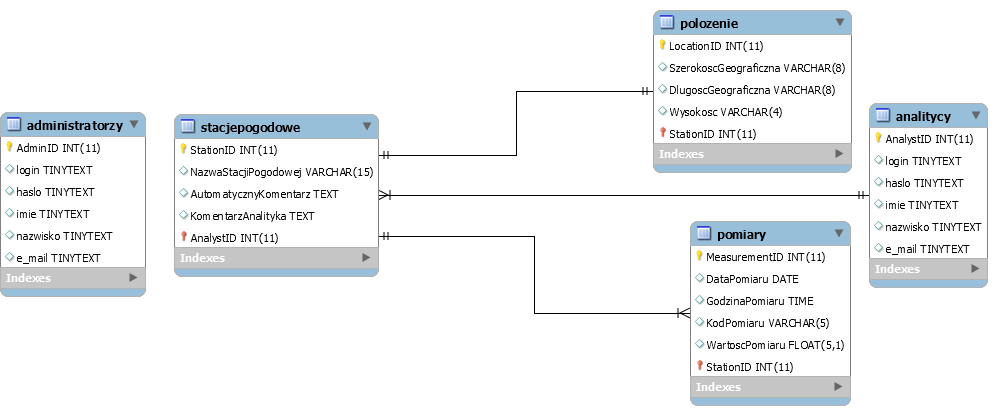
\includegraphics[width=\textwidth]{./figures/diagram_zwiazkow.png}
\caption{Diagram zależności EER}
\end{figure}

\begin{footnotesize}
\begin{itemize}
\item Stacje pogodowe (StationID)
    \begin{itemize}
    \item Nazwa Stacji Pogodowej
    \item Automatyczny komentarz (Wynik analizy danych)
    \item Komentarz analityka (Wynik analizy danych)
    \item Analityk (AnalystID)
    \end{itemize}
\item Pomiary (MeasurementID)
    \begin{itemize}
    \item DataPomiaru
    \item GodzinaPomiaru
    \item KodPomiaru
    \item WartośćPomiaru
    \item Stacja Pogodowa (StationID)
    \end{itemize}
\item Położenie (LocalizationID)
	\begin{itemize}
	\item Szerokość geograficzna
    \item Długość geograficzna
    \item Wysokość (m n.p.m.)
    \item Stacja Pogodowa (StationID)
	\end{itemize}
\item Administratorzy (AdminID)
    \begin{itemize}
    \item Login
    \item Hasło
    \item Imię
    \item Nazwisko
    \item e-mail
    \end{itemize}
\item Analitycy (AnalystID)
    \begin{itemize}
    \item Login
    \item Hasło
    \item Imię
    \item Nazwisko
    \item e-mail
    \end{itemize}
\end{itemize}
\end{footnotesize}
Kod Pomiaru jest tablicą maksymalnie 4 znaków jednoznacznie identyfikujących typ wielkości fizycznej przechowywanej w tym rzędzie:
\begin{itemize}
\item TMAX - Maksymalna dzienna/godzinowa temperatura powietrza ($^\circ C$)
\item TMIN - Minimalna dzienna/godzinowa temperatura powietrza ($^\circ C$)
\item TMID - Średnia dzienna/godzinowa temperatura powietrza ($^\circ C$)
\item HAVG - Średnia wilgotność powietrza (\%)
\item WDIR - Kierunek wiatru
\item WINT - Średnia prędkość wiatru (km/h)
\item WGUS - Prędkość wiatru w porywach (km/h)
\item PRES - Ciśnienie (hPa)
\item PREC - Opady ogólnie (deszcz, śnieg) (mm)
\item TCLD - Zachmurzenie całkowite
\item LCLD - Zachmurzenie w dolnych partiach
\item SVIS - Widoczność (km)
\end{itemize}
\newpage
\subsection{Lista funkcjonalności}
%tabelka z rolami uzytkownikow
\begin{table}[!htb]
\centering
\caption{Poziomy kompetencji klientów} 
  \resizebox{0.9\textwidth}{!}{\begin{tabular}{ | c | c | c | c |}   
    \hline
    \textbf{Klient }& \textbf{Stacje }& \textbf{Pomiary }& \textbf{Położenie }\\ \hline
    \textbf{Administrator }& owner & owner & owner  \\ \hline
    \textbf{Analityk }& owner & table.readonly & table.readonly \\     \hline
    \textbf{Użytkownik }& table.readonly & table.readonly & table.readonly  \\ \hline
  \end{tabular}}
\end{table}

\begin{table}[!htb]
\centering 
  \resizebox{0.7\textwidth}{!}{\begin{tabular}{ | c | c | c | }   
    \hline
    \textbf{Klient }& \textbf{Administratorzy }& \textbf{Analitycy}\\ \hline    
    \textbf{Administrator }& owner & owner  \\ \hline
    \textbf{Analityk }& - & - \\    \hline
    \textbf{Użytkownik } & - & - \\ \hline
  \end{tabular}}
\end{table}

Rolom przyporządkowanym do poszczególnych użytkowników przyporządkowano następujące przywileje:
\begin{itemize}
\item owner : INSERT, SELECT, UPDATE, CREATE, DELETE
\item table.readonly : SELECT
\end{itemize}

\begin{figure}[!htb]
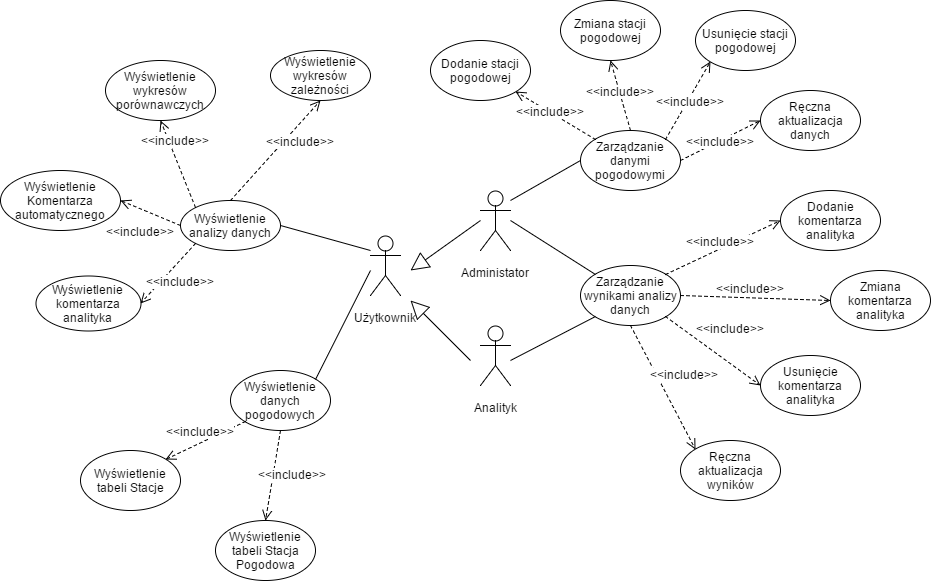
\includegraphics[width=\textwidth]{./figures/DiagramPrzypadkowUzycia.png}
\caption{Diagram przypadków użycia}
\end{figure}
 
 \newpage
\begin{small}
\begin{enumerate}
\item Użytkownik
    \begin{itemize}
    \item Wyświetlenie analizy danych
        \begin{itemize}
        \item Wykresy zależności czynników pogodowych
        \item Wykresy porównawcze warunków między stacjami
        \item Komentarz automatyczny
        \item Komentarz analityka
        \end{itemize}
    \item Wyświetlenie danych pogodowych
        \begin{itemize}
        \item Wyświetlenie tabeli Stacje
        \item Wyświetlenie tabel Stacja Pogodowa
        \end{itemize}
    \end{itemize}
\item Administrator (dziedziczy po użytkowniku)
    \begin{itemize}
    \item Zarządzanie danymi pogodowymi
        \begin{itemize}
        \item Dodanie stacji pogodowej
        \item Usunięcie stacji pogodowej
        \item Zmiana stacji pogodowej
        \item Ręczna aktualizacja danych
        \end{itemize}
    \item Zarządzanie wynikami analizy danych
        \begin{itemize}
        \item Zmiana komentarza analityka
        \item Ręczna aktualizacja wyników
        \item Odczytanie id analityka dodającego komentarz
        \end{itemize}
    \end{itemize}
\item Analityk (dziedziczy po użytkowniku)
    \begin{itemize}
    \item Zarządzanie wynikami analizy danych
        \begin{itemize}
        \item Zmiana komentarza analityka
        \item Ręczna aktualizacja wyników
        \end{itemize}
    \end{itemize}
\end{enumerate}
 
\end{small}
\end{document}